\section{\infersent{}}\label{sec:evaluation-inferSent}

% pool type
The \texttt{max} pooling type is used for the \infersent{} model, since \citeauthor{inferSent2018} 
found by conducting experiments using different pooling techniques that it was the best option.

% version/ embeddings dictionary
Initially, in this work, the \ac{glove} word embeddings were used for the \infersent{} model.
However, since the file of precomputed \acs{glove} word embeddings has a size of 5.65 \ac{gb} and thus,
slows down the model, ultimately another word embedding was used.
The time necessary to compute and insert 195 documents for specific embeddings is displayed in \autoref{fig:times_emb}.
The custom word embedding used in this work is a \ac{w2v} model trained on a selection of 195 documents from the Bahamas dataset.

% glove
\citeauthor{glove2014} state that \acs{glove} outperforms \ac{w2v} on the same corpus, 
vocabulary and window size in terms of quality and speed \cite{glove2014}.
Hence, the quality of the results obtained in this work may have suffered from using a custom \ac{w2v} instead of \acs{glove}.
However, since the computation time of the project is a crucial factor, the custom \ac{w2v} was used.

\begin{figure}%
    \centering
    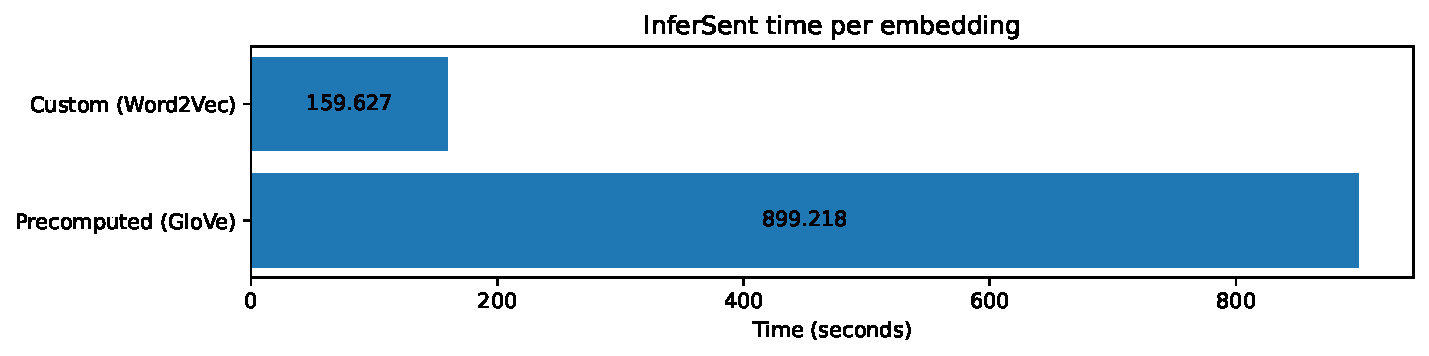
\includegraphics[width=0.6\textwidth]{images/embeddings/infersent/InferSent_time_per_embedding.pdf}
    \caption{Time necessary to calculate and insert \infersent{} embeddings for different precomputed word embeddings on a \localMaschineStats{}.
    }
    \label{fig:times_emb}%
\end{figure}
